% siminos/spatiotemp/Solutions/soluCOM.tex
% $Author: predrag $ $Date: 2021-12-24 01:25:20 -0500 (Fri, 24 Dec 2021) $

% Predrag soluCOM.tex                                           2021-02-15
%               ChaosBook.org soluCOM.tex   to here
%predrag                24mar2005
%predrag                24jan2005
%predrag                 3jan2005
%predrag                27dec2004

\section{``Center of mass'' puzzle}
\label{s:CenterOfMass}
\index{center of mass}

Some of Predrag's unpublished 2004 drafts and calculations are in
\begin{verbatim}
% dasbuch/book/FigSrc/gnu/Gallas % just a link
dasbuch/WWW/library/Gallas-chiral.pdf
dasbuch/WWW/projects/revHenon/Gallas0101305.txt  etc
dasbuch/book/Fig/COM0001011.eps  COM0001101.eps  COM000111.eps
                 COM0011.eps     COM011.eps
dasbuch/book/OldProblems/soluCOM011005.tex
\end{verbatim}

\noindent
{\em predrag/reports/referee/Gallas.txt} on the unpublished

{\em Periodic orbits are not necessarily independent from each other}

\noindent
Some of Predrag's unpublished 2004 drafts and calculations
of Jan 26, 1999 suggests many references where similar work was
published. The revised paper appeared as Gallas\rf{Gallas99} {\em
Nonlinear dependencies between sets of periodic orbits}, I believe.
\\

 {{\em Gallas-chiral.pdf}} \CBlibrary{Gallas-chiral} has the Endler-Gallas
\HenonMap\ polynomials up to period 8, and nothing else.
\\

\wwwcb{/projects/revHenon} has lots of stuff:
\begin{enumerate}
  \item
\emph{chiral.pdf} is an unfinished draft of Endler, Gallas and
Cvitanovi{\'c} paper, based on {\em Gallas-chiral.pdf}. Much of the
introduction is utterly delirious. Notation for `orbits', eq.~(10)
is redundant and the indices of $x_j$ are useless, they label roots of
different polynomials, ordered by increasing $x_j$.

Figures illustrate `chiral' orbit pairs, $A_\cl{}=0$;
 $B_\cl{}=0$ and  $C_\cl{}=0$ self-dual orbits. Fig.~4 might be
$C_\cl{}=0$ for value of $a$ other than 6.

  \item
From: Jason Alfredo Carlson Gallas (14 Jan 2005) fortran \emph{plot\_orbit.f},
generates *.eps files, see \emph{Fig-7cycles.txt},
\emph{Gallas0101305.txt}.

  \item
{\em per7.pdf} 18 period-7 orbits.

  \item
{\em chiral\_p8.pdf} 3 period-8 time-asymmetric pairs.

  \item
{\em per8.pdf}: 18 self-dual period-8 orbits (not sure that is a
complete list).

  \item
{\em FourClasses.pdf}: defines four classes of orbits under time reversal;
perhaps useful, still need to find the LaTeX file.

  \item
{\em tres.pdf}: period-6, symmetries with respect to the main diagonal
of 3 6-cycles ``corresponding to a $\sigma^3$ factor,'' plotted for $a=7$.
No idea what that is...

  \item
\emph{Gallas0101305.txt} says he does not understand me.

  \item
\emph{Predrag011304.txt}  my last attempt to explain symbolic dynamics
and why is this a time-reversal symmetry. ``Please use `time reversal'
rather than `chiral'. It is a standard part of the lore of Hamiltonian
dynamics, and especially Hamiltonian/symplectic mappings.'' Hopeless.

  \item
{\em puzzle.pdf}, {\em puzzle.tex} is January 25, 2005 version of Endler and
Gallas\rf{EG05} (submitted December 25, 2005?) that uses ChaosBook
notation - Table~1 can be used as a check on Sidney's \po s.
Other versions:
{\em puzzle011305.tex}  of 13 Jan 2005;
 {\em puzzle.tex} and {\em puzzle2dasbuch.tex} of 27 Jan 2005;

They published in {\em Reductions and simplifications of
orbital sums in a {Hamiltonian} repeller}\rf{EndGal06} without me as a
coauthor. Algebraic number expressions for periodic points
show interesting patterns, their eqs.~(22),
(23) and (28), that would not be noticed from their numerical values.

They use binary labelling also in Endler and Gallas\rf{EG05a} {\em
Conjugacy classes and chiral doublets in the {H{\'e}non Hamiltonian}
repeller}, without mentioning me or ChaosBook at all.

  \item
{\em citation.txt} and {\em puzzle.end} is the footnote which Gallas
would not accept:
{\em endnote27}~~{\em This exact equation was discovered by P.
Cvitanovi\'c during discussion and in collaboration with the authors. }

  \item
{\em old/puzzle011805.pdf} has my comments

  \item
{\em solRevHen.pdf} is extracted from
\wwwcb{/projects}, version 11.2.2, Mar 10 2005. I believe all that is
in ChaosBook, ignore.

  \item
{\em revHenon.pdf}, {\em revHenon.zip} is a template for a
\wwwcb{/projects} extracted from Jason Gallas, Predrag edited \emph{puzzle.tex},
Gallas text	removed 18 Feb 2006.
I believe no one took up the project.
\end{enumerate}

To summarize, this 2005 work agrees with current Han's work, but does not
clarify the problems we are dealing with now. The figures might be useful
as crosschecks for Sidney's \Henon\ orbits.

\bigskip

\begin{description}
\item[2021-02-16 Predrag]
% in ChaosBook.org \solution{e:CenterOfMass}{``Center of mass'' puzzle$^{**}$.}{
\PC{27dec2004}{
Extracted from the ChaosBook.org boyscout,  version of 2018-08-02 tex files.
Edited here, so eventually return to ChaosBook.
}
                                                        \toCB
Here are my notes on the work of Gallas and collaborators;
they have written many papers on
polynomial maps%
\rf{EndGal01,EndGal02,EG05,EG05a,EndGal06,Gallas18,Gallas20,Gallas20a}.
What I had contributed (unpublished, I believe) is to show Gallas
how to use time-reversal,
\refeq{EGfactor2B}, \refeq{EGfactorS} and \refeq{EGfactorP},
wrote a draft of a paper (click on
\HREF{Http://ChaosBook.org/projects/revHenon/chiral.pdf} {chiral.pdf}),
and --when he was not interested in it-- requested my traditional citation,
\begin{quote}
 This exact equation was discovered by P. Cvitanovi\'c
during discussion and in collaboration with the authors.
\end{quote}
but he refused to credit me for that, so I - what's the point - I stopped
following their papers. I remember him being stubborn in a male kind of
way. Absolutely refuses to understand binary symbolic dynamics, that what
he understands\rf{gallas_counting} to be `spatial $x\leftrightarrow{y}$
symmetry'

\begin{quote}
``[...] three algebraic conjugacy classes with respect to
a spatial reflection $R(x, y) = (y, x)$ about the $y = x$ symmetry
diagonal in phase-space.''
\end{quote}

is time reversal, and he would not try to understand ChaosBook symmetry
factorizations.  But it is quite possible that they (or younger me?) did
the right thing and quotiented the time reversal... Check the papers and
the papers they refer to.

As he has worked on this for at least 20 years, there are many details
specific to quadratic mappings that I think we can ignore here. Here is
an overview from my point of view:
Gallas \etal\ observe that
\begin{enumerate}
  \item
for polynomial mapping \refeq{cycle-polyn} the \emph{orbital sum}
\beq
\sigma_p = \sum_{i \in p} x_{p,i}
\ee{COMdef}
% \refeq{COMdef}
is a \emph{prime} cycle $p$ \emph{invariant} that satisfies a
(factorized!) polynomial equation
${\mathbb S}_\cl{}(\sigma)=0$
of the order $\cl{p}$, the period of the cycle, see for example
\refeq{Gallas20a:S_5}.

{\bf Predrag addendum}:
{\HillDet}s are \emph{symmetric polynomials} in lattice fields
$\{\field_1,\field_2,\cdots,\field_\cl{}\}$, which are, by construction,
all \emph{prime} cycle $p$ \emph{invariants}.
The {orbital sum} \refeq{COMdef} is one example.
Another one is the bilinear \refeq{HillDetHen2cycle}.

  \item
the cycle-points $\ssp_{p,i}$ of a given cycle are roots of a polynomial
\refeq{cycle-polyn} of order  $\cl{p}$, see for example
\refeq{Gallas20a:c_5,1}. This is remarkable, as higher iterates of a
polynomial mapping are polynomials of a horrendous order.
  \item
time-reversal invariance (my interpretation, not theirs) induces the
\beq
{\mathbb S}_\cl{} = C_\cl{}^2 D_\cl{} N_\cl{}
\,.
\ee{EGfactorS}
factorization of such polynomials, where D=`diagonal'
class, N=`non-diagonal' class, and `C=`chiral' class, see below.

For me this is the key result.
\end{enumerate}

This ${\mathbb S}_\cl{}$ is very smart, as it has a zero for every
\emph{prime} orbit. Perhaps we can bring this to a full square, by
including the boundary into the definition of the temporal lattice
fundamental domain, with $(C D N)$ {\orbit}s (perhaps in the Fourier
space - they talk about `cyclotomic polynomials')
\beq
{\mathbb S} = \frac{(C D N)^2}{D N}
\ee{EGfactorSincExcl}
by taking care of the temporal fundamental domain boundary by the
inclusion-exclusion principle \refeq{KlaRot97(2.1)}, and proceed to
zeta-function factorization in the spirit of \refeq{Lat-LapSqrt},
\refeq{tildejMorbRel}, for each { Hamiltonian {\Henon}} cycle separately.

I believe factorization \refeq{EGfactorSincExcl} should apply to
\po s of \emph{any time-reversible} mapping, not just \Henon\ and \templatt,
but the `N class' worries me.

 \refeq{Lat-LapSqrt}

\bea
\left(\shift-\unit\right)
 &=&
\tilde{\shift}\tilde{\partial}
     % \left(\tilde{\shift}-\tilde{\shift}^{-1}\right)
    \continue
\left(\shift^{-1}-\unit\right)\left(\shift-\unit\right)
 &=&
    - \tilde{\partial}^2
  = \Box
    %\left(\tilde{\shift}-\tilde{\shift}^{-1}\right)^2
 \label{COM:LapSqrt}\\
\jMorb  &=& \Box - \mu^2\unit
         =
\left(
\tilde{\partial} + \mu\unit  %\left(\tilde{\shift}-\tilde{\shift}^{-1}\right)
\right)
\left(
\tilde{\partial} - \mu\unit  %\left(\tilde{\shift}-\tilde{\shift}^{-1}\right)
\right)
    \continue
\tilde{\jMorb}
     &=& \tilde{\partial} - {\mu}\unit
    \,=\,
    \tilde{\shift} - \mu\unit -\tilde{\shift}^{-1}
\nnu
\eea


\item[2021-02-19 Predrag]
Gallas\rf{gallas_counting} {\em Counting orbits in conjugacy classes of
the {{\Henon} Hamiltonian} repeller} counts the numbers $C_\cl{}$,
$D_\cl{}$, $N_\cl{}$ of \refeq{EGfactorSincExcl} {\orbit}s
(switched to calling `prime cycles' orbits, like Gallas does) in each class, for any
arbitrary period $\cl{}$.

$D_\cl{}$ is sensible, relatively simply related to the number of points on the
time-reversal diagonal; one expects something like that for any system.

 $N_\cl{}$ is funky,  has to do with the parabola symmetry
line, might be what we call "dynamical".

$C_\cl{}$ is just the remainder $M_\cl{}-D_\cl{}-N_\cl{}$:
$C_1=\cdots=C_5=0$, and then (Gallas Table~1), starting with $C_6/2=1$:
\beq
  1,2,6,14,30,62,127,252,500,968, 25446,\cdots
\ee{gallas_counting:tab1}
This is not in \emph{On-Line Encyclopedia of Integer Sequences}
\HREF{https://oeis.org/} {OEIS},
(It is close to \HREF{https://oeis.org/A000918} {OEIS:A000918} A000918 		
$a(n) = 2^n - 2$ and $a(n+1) = 2 + 2a(n)$)
so it has to be reverse engineered to find the $\tilde{N}_\cl{}$, the numbers of
periodic points of the yet to be written down $\sqrt{\mbox{\Henon\ map}}$.


The number of $C_\cl{}/2$ periodic points:
\[
  \tilde{N}_6= 1*6=6,
  \tilde{N}_7= 2*7=14,
  \tilde{N}_8= 6*8=48,
  \tilde{N}_9= 14*9=126,
\]
Actually, $ \tilde{N}_\cl{}= \cl{}\,C_\cl{}/2+\cl{}(D_{2\cl{}}+N_{2\cl{}})$
looks more sensible
\[
  \tilde{N}_6= **,
  \tilde{N}_7= 2*7+1=5,
  \tilde{N}_8= 6*8+1=19,
  \tilde{N}_9= 14*9+2*2+1=61,
\]


MacKay had these numbers already
listed in Table 1.2.3.5.1 of his 1982 PhD thesis\rf{Bmack93}
\CBlibrary{Bmack93}.

%%%%%%%%%%%%%%%%%%%%%%%%%%%%%%%%%%%%%%%%%%%%%%%%%%%%
\begin{table}
\begin{tabular}{c|rrrrr|rrrrr|rrrrr}
$\cl{}$ &  1 &  2 &  3 &  4 &  5 &
       6 &  7 &  8 &  9 & 10 &
      11 \\%& 12 & 13 & 14 & 15 \\
\hline
$N_\cl{}$ &  2 &  4 &  8 & 16 &  32 &
       64 &  128 &  256 & 512 & 1024 &
      . % \\%& 12 & 13 & 14 & 15 \\
             \rule[-1ex]{0ex}{3.5ex} \\
$M_\cl{}$ &   2 &   1 &   2 &  3 &  6 &
         9 & 18 &  30 & 56  & 99 &
       186 &  %% &     &     &
\end{tabular}
\bigskip
\caption{\label{tab:HamHenon}
{\Lattstate}s and %{prime}
orbit counts for the ${a}=6$ \Henon\ map.
Compare with the golden (Fibonacci\rf{BaNeRo13}) cat map \reftab{BaRoWe08fib-tab}
and \refeq{zetasqrt-N}.
}
\end{table}
%%%%%%%%%%%%%%%%%%%%%%%%%%%%%%%%%%%%%%%%%%%%%%%%%%%%
%

%%%%%%%%%%%%%%%%%%%%%%%%%%%%%%%%%%%%%%%%%%%%%%%%%%%%
\begin{table}
\begin{tabular}{c|rrrrr|rrrrr|rrrrr}
$\cl{}$ &  1 &  2 &  3 &  4 &  5 &
       6 &  7 &  8 &  9 & 10 &
      11 & 12 & 13 & 14 & 15 \\
\hline
$\tilde{N}_\cl{}$ &   2 &   2 &   4 &   4 &   8 &
         8 & 16 &  16 & 32 &  32 &
        . & . & . & . & . \rule[-1ex]{0ex}{3.5ex} \\
$\tilde{M}_\cl{}$  &  3 &   . &   . &   . &    . &
             &   . &   . &   . &   . &
           . &  . &   . &   . & .
\end{tabular}
\bigskip
\caption{\label{goldenHen}
    Temporal {\lattstate}s and %{\orbit} counts for the
    $\mu=1$  golden cat map.
    See \refeq{zetasqrt-N} and the counting of walks on
    the ``half time-step'' Markov graph \reffig{fig:HLHalfStepMarkov}.
    }
\end{table}
%%%%%%%%%%%%%%%%%%%%%%%%%%%%%%%%%%%%%%%%%%%%%%%%%%%%


Assuming that \refeq{tildejMorbRel} applies, we can compute
$\tilde{N}(\mu)_{\cl{}}$ from ${N}(s)_{\cl{}}$
\bea
2^n &=& \tilde{N}(\mu)_{\cl{}}^2
    \,,\quad
n \mbox{ odd}
    \continue
2^{\cl{}} &=& \tilde{N}(\mu)_{2\cl{}}
    \,,\quad
n \mbox{ even}
\,.
\label{tildejMorbRelHen}
\eea


\item[2004-12-27 Predrag]
These extracts from ChaosBook.org are meant to complement and perhaps add
to the Endler and Gallas explanation\rf{EG05} of the ``center of mass''
puzzle for the cycles listed in \reftab{gv:cycles}, first observed
numerically by G.~Vattay in \refref{BCISV93}.

\item[2016-09-19 Predrag]
    \PC{2021-02-15} {Copied from {\em DBblog.tex} - return eventually,
    as there are edits here. Not sure where the next few paragraphs came from.}

We present exact formulas solving the problem of partitioning the total
number $M_k$ of period-k orbits of the area-preserving {\HenonMap} into the
number of orbits building its three possible conjugacy classes. The
formulas are valid for any arbitrary period n. They are derived with
combinatorial methods, by an application of the
number-theoretic Moebius inversion formula to a key problem in physics and
dynamical systems. A handy MAPLE implementation of the formulas is also
provided.

A number of orbital symmetries and asymmetries computed analytically and
systematically for the Hamiltonian (area-preserving) $b=-1$ limit of the
{\HenonMap}
have been studied in \refrefs{EG05a,EndGal06}.

Endler and Gallas\rf{EG05} prefer the equivalent, rescaled form $x\to x/a$
of the Hamiltonian {\HenonMap} \refeq{HenonLapl}:
\beq
  x_{n-1} - 2 x_n + x_{n+1} +  (x_n + 2) x_n = a
\,,
\ee{EG05:ar_pres}
They write:
``
The advantage of this equation is that it generates \emph{monic} minimal
polynomials, i.e. polynomials having 1 as the leading coefficient.
''

The key result
reported was the existence of a natural segregation of all orbits into
three algebraic conjugacy classes   with respect to a spatial reflection
R(x,y)=(y,x) about the y=x symmetry diagonal in \statesp. Under
reflection, every periodic orbit was found to fall into one of
three classes:
\begin{itemize}
  \item[D]
diagonal class, formed by symmetric orbits with points on the
time-reversal symmetry diagonal.
An odd period symmetric cycle has an odd number of points on the boundary,
see \reffig{COMcycles}\,(a).
An even period symmetric cycle has an even number of points on the boundary,
see \reffig{COMcycles}\,(b).
  \item[N]
non-diagonal class, formed by self-symmetric orbits without   points on
the symmetry diagonal, see \reffig{COMcycles}\,(c).
  \item[C]
chiral class, formed by pairs of asymmetric cycles that map into each
other, see \reffig{COMcycles}\,(d,e).
\end{itemize}

%%%%%%%%%%%%%%%%%%%%%%%%%%%%%%%%%%%%%%%%%%%%%%%%%%%%%%%%%%%%
% Date: Thu, 13 Jan 2005
% From: Predrag Cvitanovic <predrag.cvitanovic@physics.gatech.edu>
% To: Jason Alfredo Carlson Gallas <jgallas@if.ufrgs.br>
\FIG{
(a)
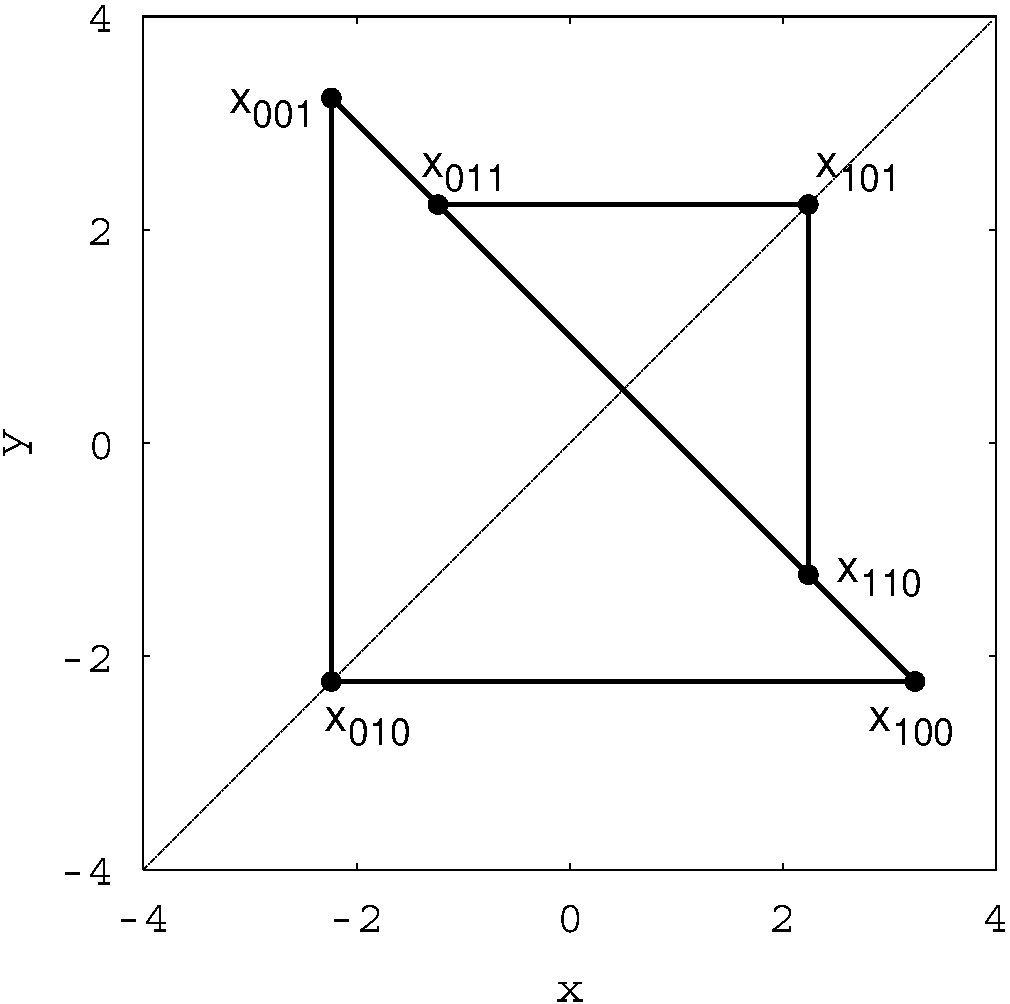
\includegraphics[width=0.30\textwidth]{COM011}
 \;
(b)
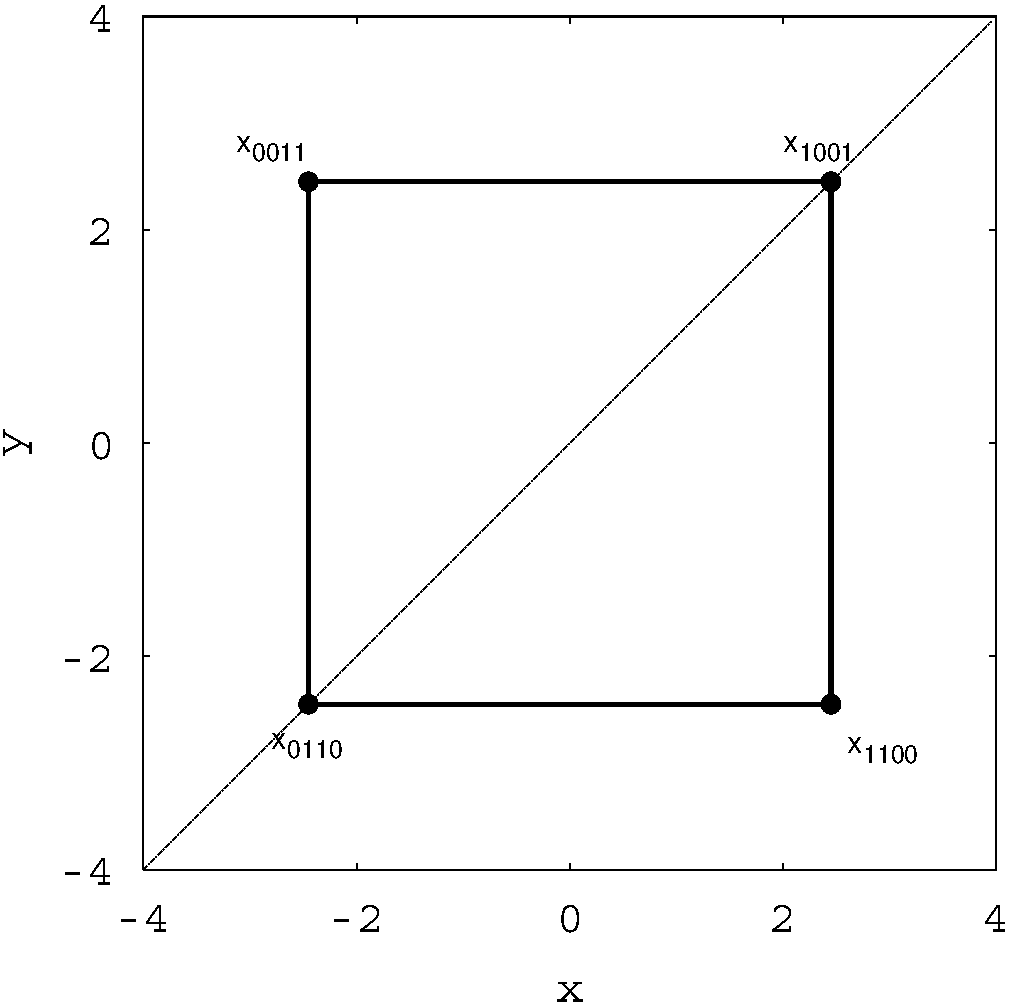
\includegraphics[width=0.30\textwidth]{COM0011}
 \;\\
(c)
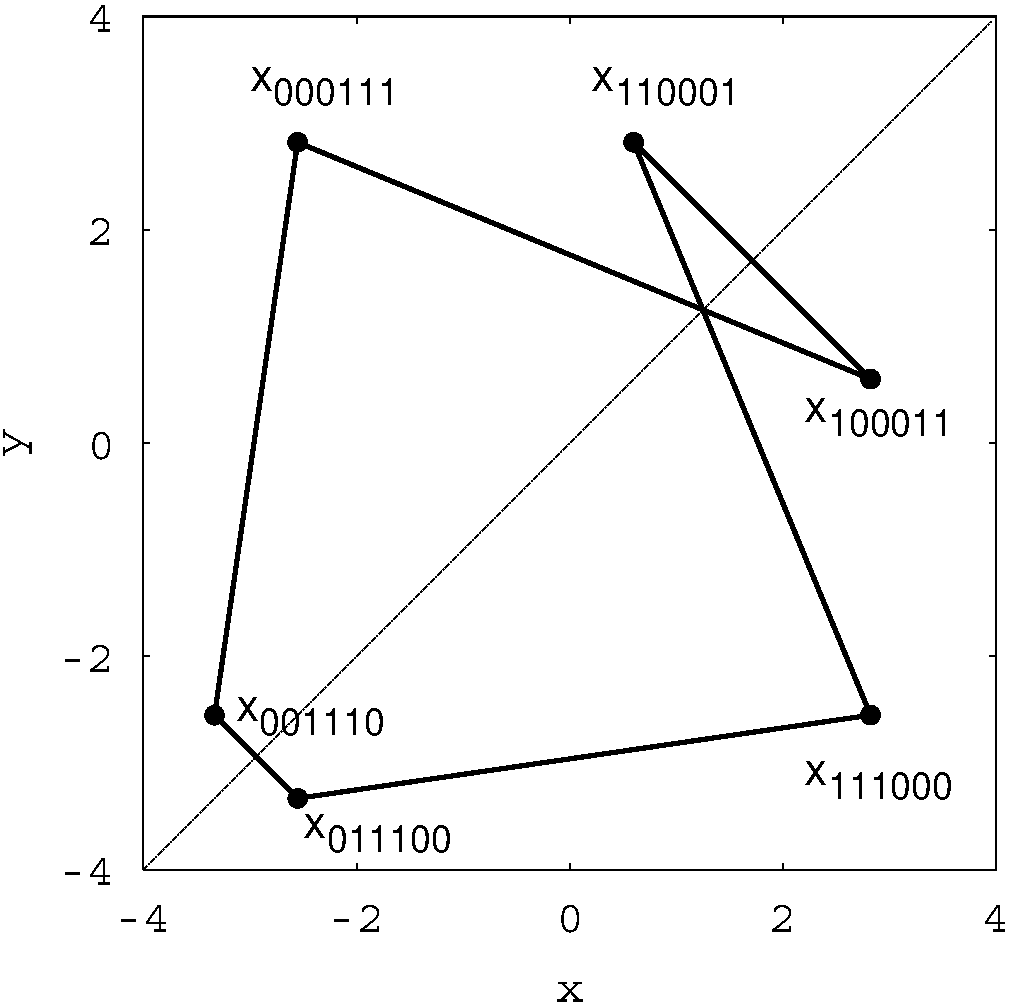
\includegraphics[width=0.30\textwidth]{COM000111}
\\
(d)
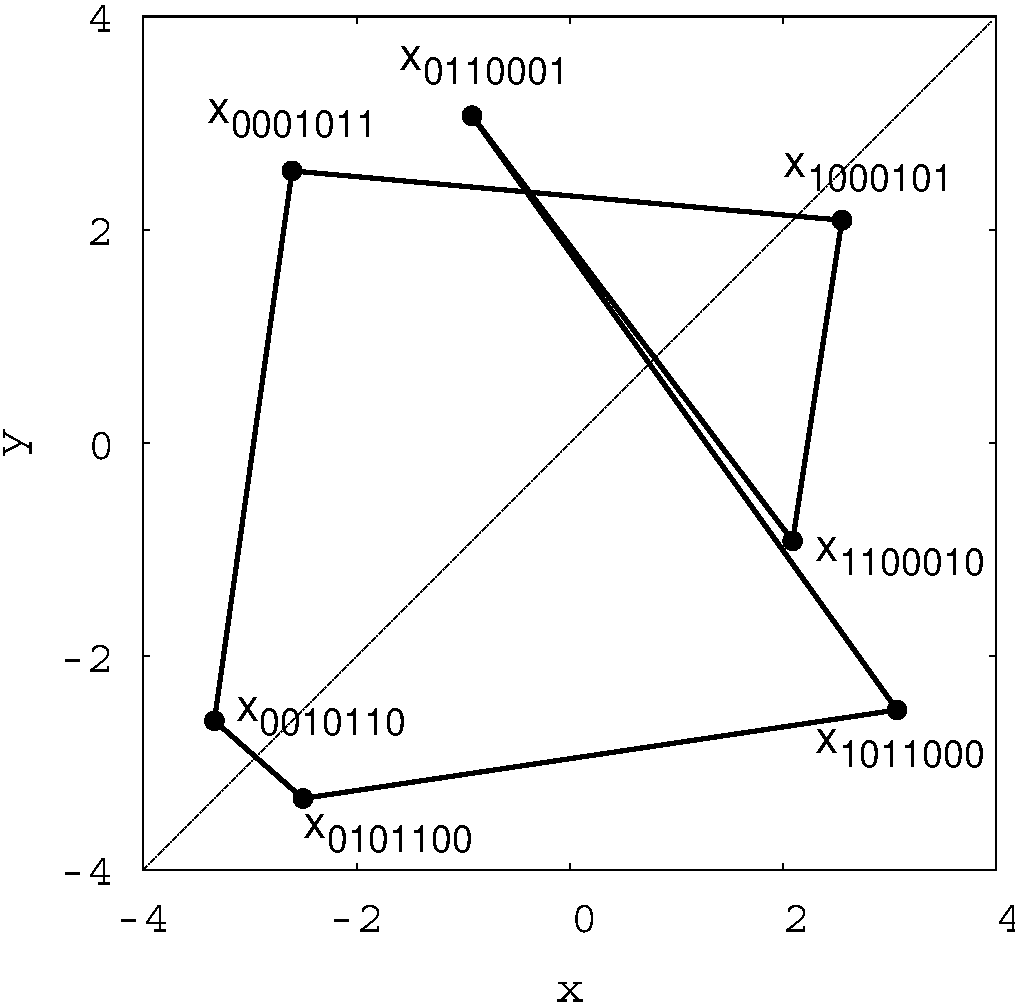
\includegraphics[width=0.30\textwidth]{COM0001011}
 \;
(e)
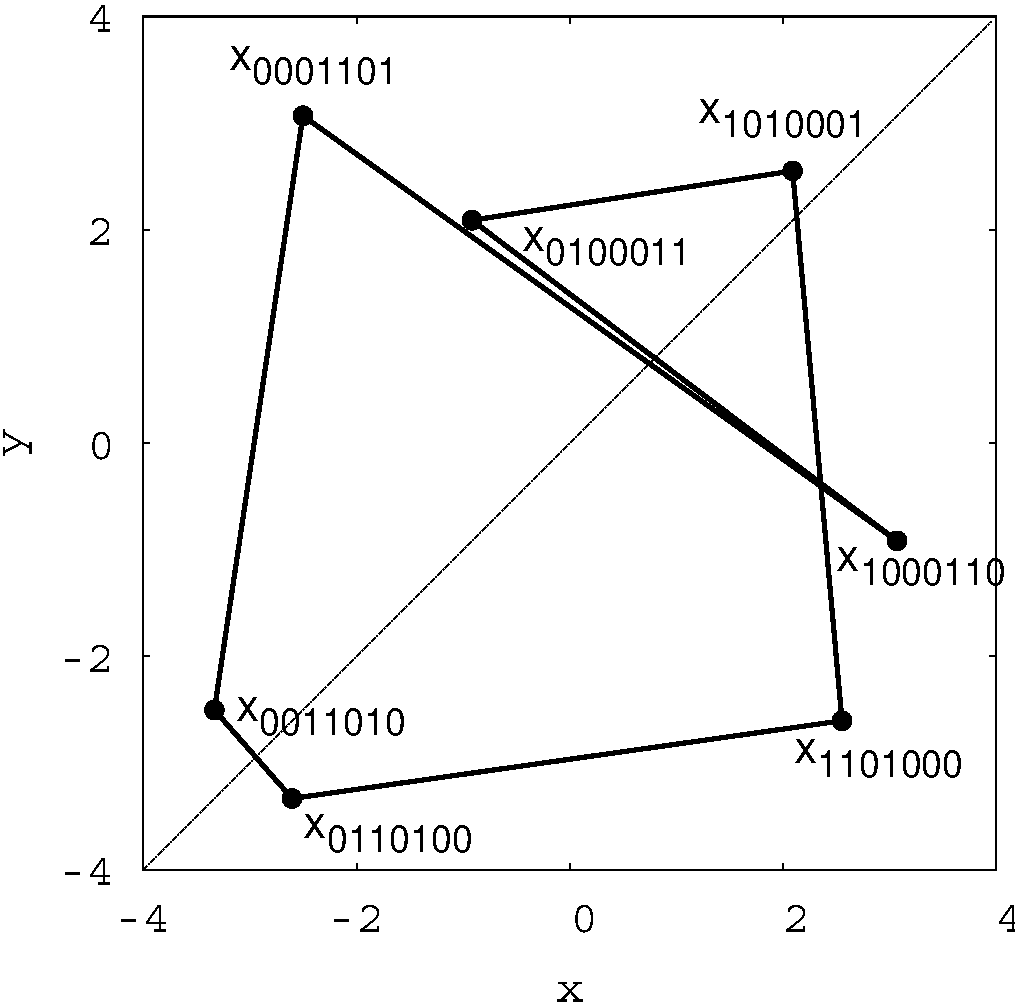
\includegraphics[width=0.30\textwidth]{COM0001101}
}{}{
\Po s of the Hamiltonian {\HenonMap} \refeq{e_ar_pres}:
(a)
An odd-period orbit can have a point on the boundary, and thus belong to the
diagonal class D. Example: the 3-cycles \cycle{001}, \cycle{011}.
(b)
An even-period orbit can have two points on the boundary, and thus belong to the
diagonal class D. Example: the 4-cycle \cycle{0011}.
(c)
An even-period orbit can belong to the non-diagonal class N.
Example: the 6-cycle \cycle{000111}, with no points on the boundary.
(d)
Almost all longer orbits are asymmetric, `chiral' class C.
Example: the 7-cycle \cycle{0001011}, and
(e)
its partner \cycle{0001101} under flip across the diagonal and
time-reversal. Under the time reversal periodic points symbol sequences
are mirrored into their symmetry partners point by point.
For \catlatt\ examples, see
\reffig{fig:HLPeriodicOrbitsA},
\reffig{fig:HLPeriodicOrbitsB},
\reffig{fig:HLSymmetric4CyclesA},
\reffig{fig:HLSymmetric4CyclesB},
\reffig{fig:HLAllCyclePoints}.
}{COMcycles}
%%%%%%%%%%%%%%%%%%%%%%%%%%%%%%%%%%%%%%%%%%%%%%%%%%%%%%%%%%%%%

Each class contains a characteristic algebraic signature embodied by a
specific orbital decompositions (factorizations)\rf{EG05a}. The orbital
segregation is independent of the control parameters and is specially
interesting for $a_h >5.69931\cdots$, the value beyond which there is a
complete Smale horseshoe and all orbits are real.
This Letter  reports exact analytical expressions
that count the numbers $C_n$, $D_n$, $N_n$ of
orbits in each class, for any arbitrary period $n$.

%%%%%%%%%%%%%%%%%%%%%%%%%%%%%%%%%%%%%%%%%%%%%%%%%%%%%%%
\begin{figure}
  \centering
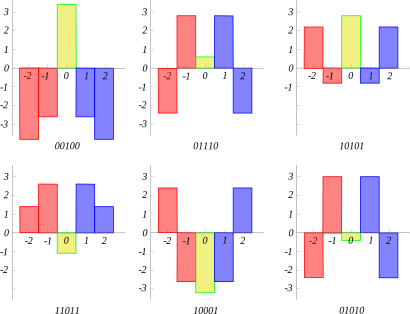
\includegraphics[width=0.95\textwidth]{PChenlatt5cyc} % from HL1dLattRefl0.svg
~~~~~~~~
% 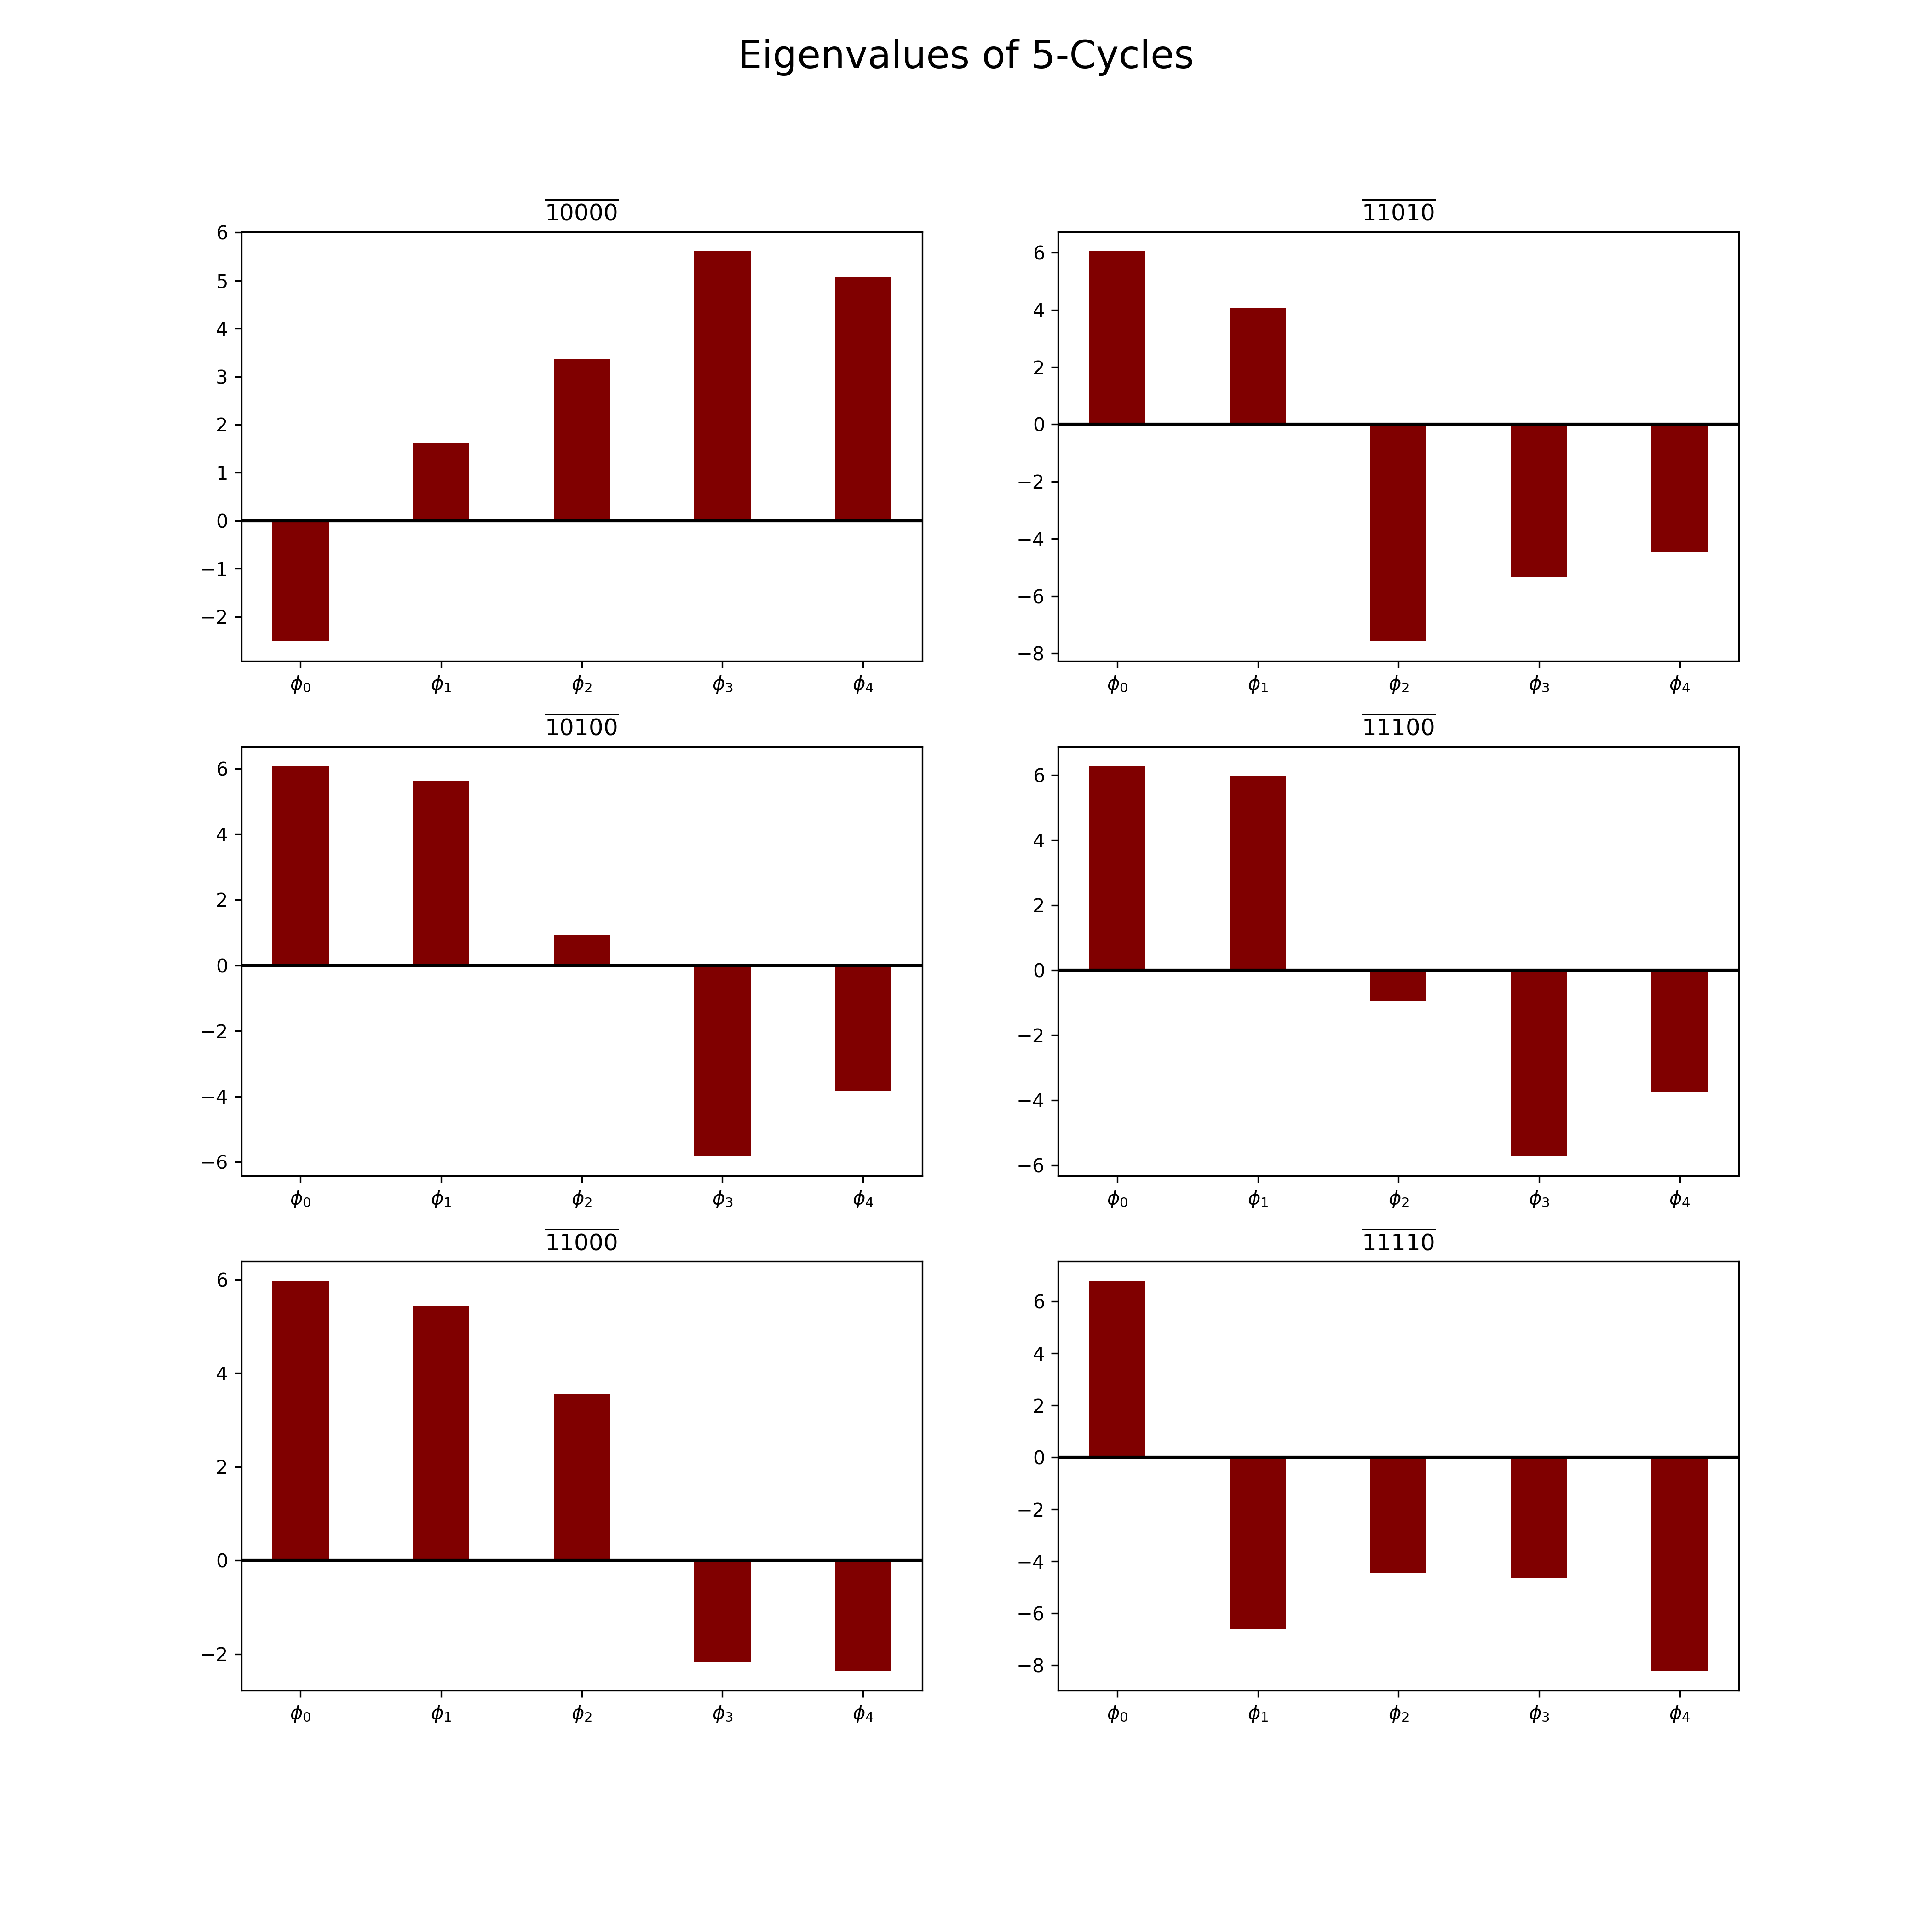
\includegraphics[width=0.45\textwidth]{SVW5eigen}
  \caption{
\Henlatt\ \refeq{Henlatt-2-step}, $a=6$:
Odd period \refeq{reflSymOdd} $\cl{}=5$ {\lattstate}s
$
\cycle{\ssp_{-2} \ssp_{-1} \sitebox{\ssp_0}\,\ssp_1 \ssp_2 |}
$
of \reftab{tab:HenCycD5},
plotted as in
\reffig{fig:symmLattStates}.
Compare also with forward-in time plots of \reffig{fig:EG05aCyc5}.
They are all reflection symmetric, with
the fixed lattice field $\sitebox{\ssp_0}$ colored gold. Note that the
symbolic dynamics is given by the signs of lattice site fields.
The most striking feature of these {\lattstate}s is how far is $a=6$
\henlatt\ from a $0\leftrightarrow1$ symmetry: stretching close to
$\cycle{0}$ constant {\lattstate} is much stronger than close to the
almost marginal $\cycle{1}$ constant {\lattstate}. Probably for somewhat
lower bifurcation value of $a$ than the `critical' value
$a_h=5.69931\cdots$, the fixed lattice sites $\sitebox{\ssp_0}$ for
$\cycle{01110}$ and $\cycle{01010}$ coalesce and vanish, so the
bifurcation happens on the even symmetry site.
{\color{red}If anybody ever gives some thought to {\jacobianOrb}
eigenvalues of \reffig{SVW5CycHamHen}\,(right), the corresponding
eigenvectors might illuminate this point.} As $a\to\infty$ I expect this
symmetry to be restored.
}
\label{fig:PChenlatt5cyc} % started with {SVW5CycHamHen}
\end{figure}
%%%%%%%%%%%%%%%%%%%%%%%%%%%%%%%%%%%%%%%%%%%%%%%%%%%%%%%

%%%%%%%%%%%%%%%%%%%%%%%%%%%%%%%%%%%%%%%%%%%%%%%%%%%%%%%%%%%%%%
\begin{table} %[ht]
\caption{\label{tab:HenCycD5} % extracted from {tab:orbitdet}
    The {\henlatt} period-5 and -6 symmetric {\lattstate}s of type
    \reffig{fig:symmLattStates}\,(b), with symmetry indicated in the
    $\Refl$-reflection format \refeq{symmCycD5Refl}. %{HLsymmCycD5}.
    For odd $\cl{}=2m+1$, symmetric orbits reduce to {\brick}s of length $m+1$.
    For even $\cl{}=2m$, their lengths are either $m+1$ or $m$.
    The period-5 {\lattstate}s are plotted in \reffig{fig:PChenlatt5cyc}
    (to supersede \reffig{SVW5CycHamHen}\,(left)).
    There is no asymmetric period-5, the first $\Cn{\cl{}}$ asymmetric pair is
    period-6.
    Indicated: the binary code $\Ssym{j}$ of the field $\ssp_j$
    at the lattice site $j=0,1,2,3,4$.
         }
\centering
\begin{tabular}{|lll|} % right alligned columns (2 columns)
%\hline\hline %inserts double horizontal lines
\hline
 \Cn{5}  & $\ssp_{-2} \ssp_{-1} \sitebox{\ssp_0}\,\ssp_1 \ssp_2 |$ & \Dn{5}
\\[0.5ex]
 $11110$ & $11\,\sitebox{0}\,11\,|$ & $\sitebox{0}\,11\,|$\\
 $00011$ & $10\,\sitebox{0}\,01\,|$ & $\sitebox{0}\,01\,|$\\
 $00101$ & $01\,\sitebox{0}\,10\,|$ & $\sitebox{0}\,10\,|$\\
 $00001$ & $00\,\sitebox{1}\,00\,|$ & $\sitebox{1}\,00\,|$\\[0.5ex]
 $11010$ & $10\,\sitebox{1}\,01\,|$ & $\sitebox{1}\,01\,|$\\
 $11100$ & $01\,\sitebox{1}\,10\,|$ & $\sitebox{1}\,10\,|$\\
[1ex]
\hline
\end{tabular}
~~~~
\begin{tabular}{|lll|} % next table
\hline
 \Cn{6}  & $\ssp_0 \ssp_1 \ssp_2 \ssp_3 \ssp_4 \ssp_5$ & \Dn{6}
\\ [0.5ex]
 $001011$ & $001011$ & $001011$\\
 $110100$ & $110100$ &  \\
\hline
 & $\sitebox{\ssp_0} \ssp_1 \ssp_2 \sitebox{\ssp_3} \ssp_2 \ssp_1$ &
\\ [0.5ex]
 $010001$ & $\sitebox{0}\,10\,\sitebox{0}\,01$ & $\sitebox{0}\,10\,\sitebox{0}$\\
 $011111$ & $\sitebox{0}\,11\,\sitebox{1}\,11$ & $\sitebox{0}\,11\,\sitebox{1}$\\
 $001110$ & $\sitebox{0}\,01\,\sitebox{1}\,10$ & $\sitebox{0}\,01\,\sitebox{1}$\\
 $100000$ & $\sitebox{1}\,00\,\sitebox{0}\,00$ & $\sitebox{1}\,00\,\sitebox{0}$\\
 $101110$ & $\sitebox{1}\,01\,\sitebox{1}\,10$ & $\sitebox{1}\,01\,\sitebox{1}$\\
\hline
 & $ \ssp_0  \ssp_1 \ssp_2 | \ssp_2 \ssp_1 \ssp_0|$ &
\\ [0.5ex]
 $001100$ & $001|100|$ & $|001|$\\
 $011110$ & $011|110|$ & $|011|$\\
[1ex]
\hline
\end{tabular}
\end{table}
%%%%%%%%%%%%%%%%%%%%%%%%%%%%%%%%%%%%%%%%%%%%%%%%%%%%%%%%%%%%%%

%%%%%%%%%%%%%%%%%%%%%%%%%%%%%%%%%%%%%%%%%%%%%%%%%%%%%%%%%%%%
\FIG{
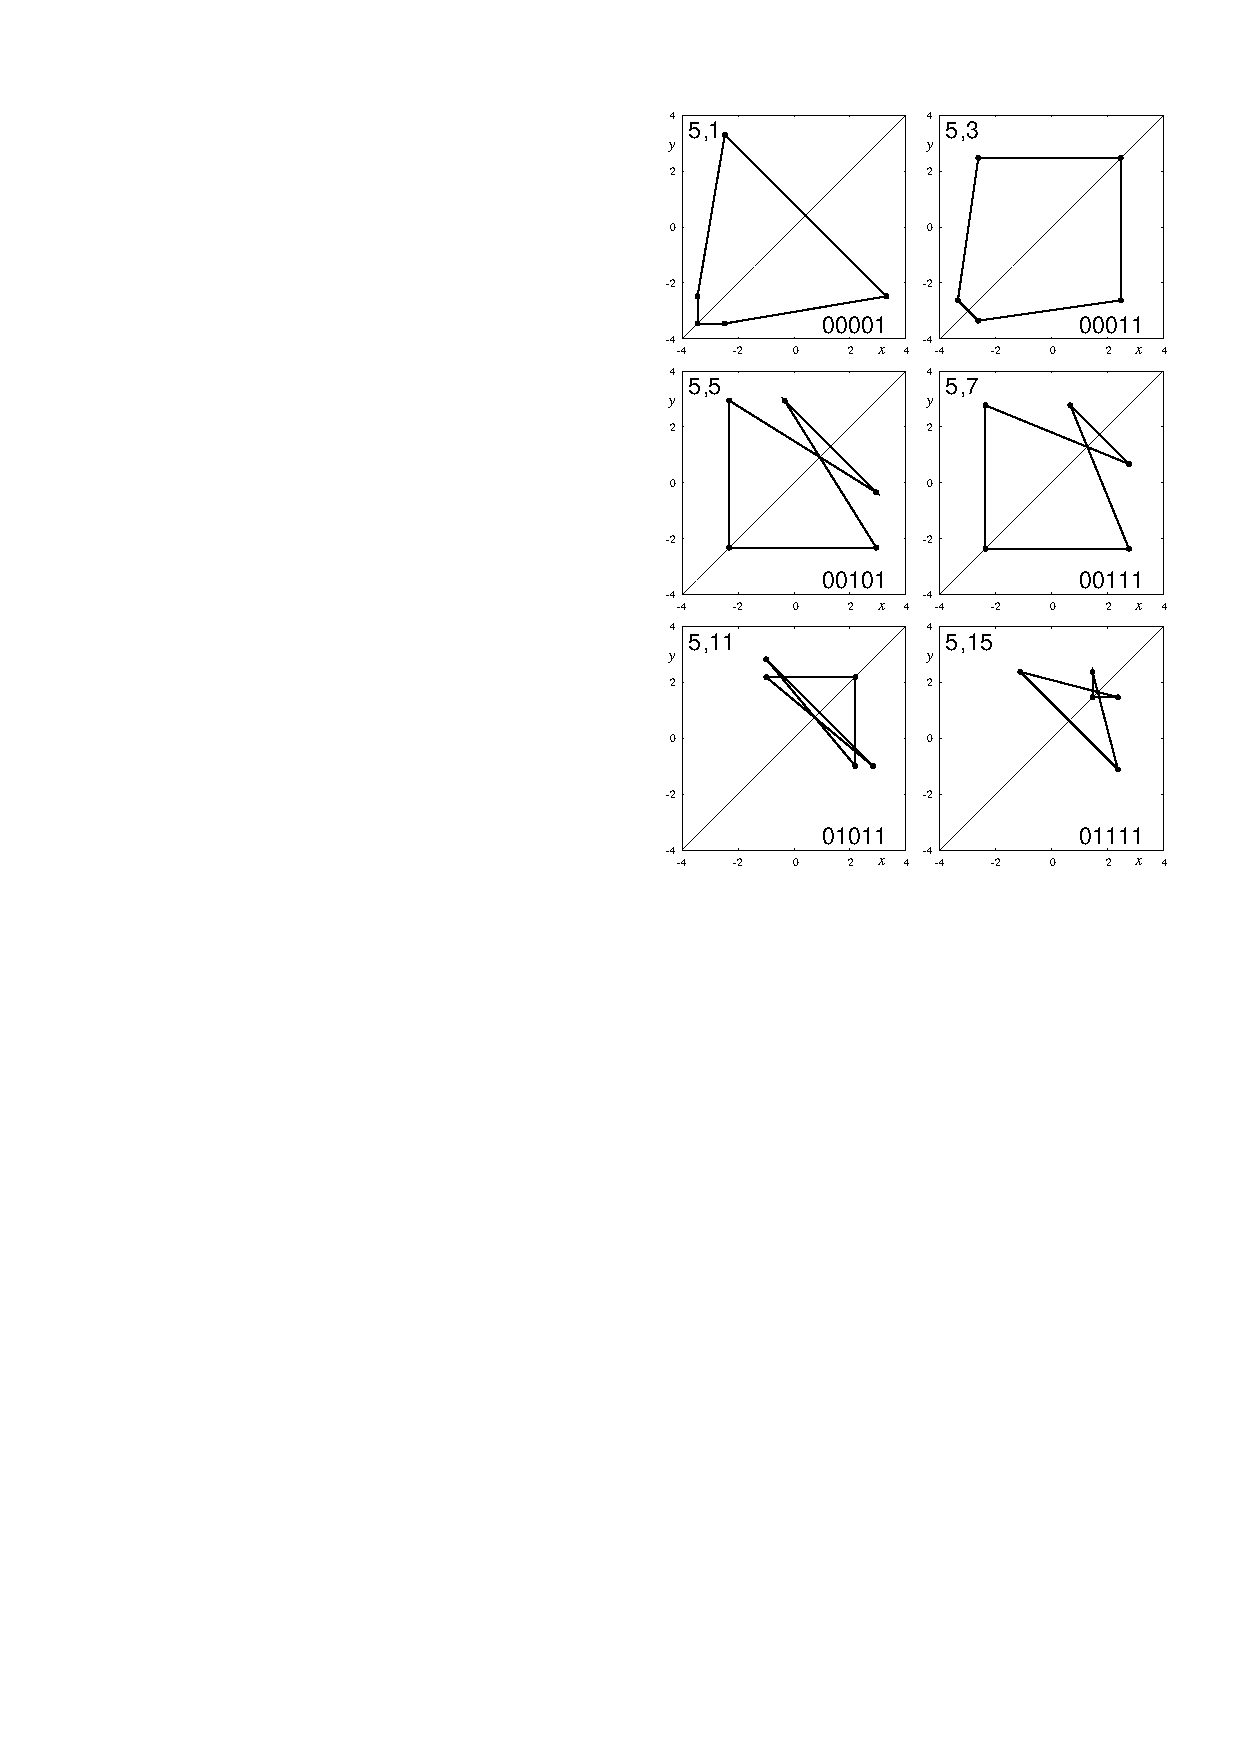
\includegraphics[width=0.60\textwidth]{EG05aCyc5}
}{}{
The 6 period-5 orbits are of Engler-Gallas class D (here called odd
period symmetric cycles $(o)$, see \refeq{reflSymOdd}): they are
symmetric under reflection across the diagonal, have a single point on
it, corresponding to 2 successive field values of an even-reflection pair.
Compare with the {\lattstate} plots of \reffig{fig:PChenlatt5cyc}.
The pairs 5,1 \& 5,3 and 5,1 \& 5,3 have an additional symmetry under
reflection and stretch (\PCedit{Predrag: what is that? I do not see it})
across the other diagonal.
%All six period-5 cycles are of class D:.
%They are symmetric under reflection about the diagonal shown. The pairs
%5,1 \& 5,3 and 5,5 \& 5,7 have an additional symmetry under reflection and
%stretch about the other diagonal.
%From \refref{EG05a}.
}{fig:EG05aCyc5}
%%%%%%%%%%%%%%%%%%%%%%%%%%%%%%%%%%%%%%%%%%%%%%%%%%%%%%%%%%%%%

                                                        \toCB
The problem of counting periodic orbits and its partitions is among the
first problems that one needs to address%
\rf{ChAnPi85,brucks,Lutzky88,Lutzky93,BLMS91,XH94,CheLou97,BriPer05}. For
the paradigmatic quadratic map it was addressed very early by
\HREF{https://en.wikipedia.org/wiki/Pekka_Myrberg} {Myrberg}, in what
appears to be one of the first applications of computers to
dynamics\rf{Myrberg58a,Myrberg58b,Myrberg59,Myrberg62,Myrberg63}. Apart
from counting orbits, he knew well how to exploit symbolic dynamics and
what was later named ``itineraries'' and ``kneading
sequences''\rf{MilThu88} to efficiently tabulate parameters with no less
than 11 digits of accuracy. The problem of counting orbits for the
{\HenonMap} was also addressed very early, in a pioneering work by
Sim{\'o}\rf{Simo79} using an approach centered in the strange attractor
creation/destruction.

The direct combinatorial problem of determining the partitions  $C_n$,
$D_n$, $N_n$  individually seems to be very hard. However there is an
efficient way of getting indirectly to them by counting the orbital
points lying on symmetry axis of the problem. This is what we do. The
approach is a nice application of enumerative combinatorics and the
number-theoretic Moebius inversion formula to a key problem in physics
and dynamical systems. Several complementary aspects of combinatorial
dynamics are discussed in \refref{AlLlMi00}.

\item[2021-02-18 Predrag]
\PCedit{Predrag: as the logistic map \refeq{Gallas20a:qm} is not invertible
map, I expect no information about the time reversal factorization from this
group of papers:}

Gallas\rf{Gallas18}
{\em Equivalence among orbital equations of polynomial maps}
 \arXiv{1809.05399}

Gallas\rf{Gallas20} {\em Orbital carriers and
inheritance in discrete-time quadratic dynamics} \arXiv{2008.01073}:

[...] may be all conveniently extracted from
just a single mathematical object, a polynomial called an
{\sl orbital carrier}, see for example \refeq{Gallas20a:S_5}.
All {\orbit}s may be encoded simultaneously by a single carrier,
with $p$ {\orbit} parameterized by the orbital sum $\sigma_p$.

recurrence

from  Pincherle's relation%\cite{Gautschi}
%\begin{equation}
% T_{\ell}(x) =  \left(\frac{x-\sqrt{x^2-4}}{2}\right)^{\ell}
%             + \left(\frac{x+\sqrt{x^2-4}}{2}\right)^{\ell},
%      \qquad \ell=0, 1, 2, \dots.
%\end{equation}


Sim{\'o}\rf{Simo79} {\em On the {H{\'e}non-Pomeau} attractor}
is a very fine early paper. Cite it in \Henon\ remark.
No mention of symmetry lines, though.

MacKay\rf{Bmack93} 1982 PhD thesis, published as
{\em Renormalisation in Area-preserving Maps} has a chapter on
reversible maps. Do cite in our paper(s).

The theory comes from deVogelaere\rf{DeVogelaere58} {\em On the structure
of symmetric periodic solutions of conservative systems, with
applications} (1958)

\end{description}
%%%%%%%%%%%%%%%%%%%%%%%%%%%%%%%%%%%%%%%%%%%%%%%%%%%%%%%%%%%%%%%%%%

\paragraph{{\Orbit}s and periodic points}

A \emph{periodic point} is a
solution $(x,\cl{})$, $x \in \reals^{d}$,
$\cl{} \in \integers$ of the {\em periodic orbit condition}
\index{periodic!orbit condition}
\beq
x = f^\cl{}(x)
\ee{COM:periodic}
for a given mapping $f$.
Each periodic point
$x=x_{p,i} \in p$
belongs to a \emph{time orbit}, a \emph{{\orbit}} $p$ of period $\cl{p}$,
and its  $\cl{p}$ distinct images
\[
f^k(x_{p,i})=x_{p,i+k}\,,\quad i+k \;\mbox{mod}\; \cl{p}
\]
are the successive periodic points
along the cycle.

A {\em {\orbit}}
\index{cycle!prime}
$p$ of period $\cl{p}$ is
a single traversal of the orbit.


We list the number of {\orbit}s up to length 10
for the 2-letter complete symbolic dynamics
in \reftabs{COM-t-mal-1}{COM-t-mal-78}.
% restore     (see \reftab{t-symm-3}).

%
% S = S_\asym^2 S_\sym S_b
% \refeq{EGfactorS}
\PC{27dec2004}{\reftab{COM-t-mal-78} derived from knead.tex} %, \refchap{c-knead}}
\PC{27dec2004}{extracted from smale.tex} %, \refchap{c-smale}}
%Predrag               27dec2004
%
%\index{H\'enon map}
%\index{map!H\'enon}
%For parameter $a$ sufficiently large the {\HenonMap} \refeq{eq2.1a} is
%another
%explicit example of a complete Smale horseshoe. %\rf{smale}.
%
% \noindent
% {\large\bf Hamiltonian {\HenonMap}}
% \\
% \PC{27dec2004}{included in  \refexam{exmp:HamHenonMap}}
% {[EG]}
%
% For definitiveness, in numerical calculations we shall fix here (arbitrarily)
% the stretching parameter value to $a=6$, a value large enough to guarantee
% that all roots of  $0=f^n(x)-x$ (periodic points) are real.
%
Consider the $n$-periodic point condition $0=f^n(x)-x$. This
polynomial of order $2^n$ has zeros at all
shorter, period $d$ {\orbit}s  if $d$ is a divisor of $\cl{}$.
Dividing those out, we arrive at the polynomial\rf{Milnor99}
\index{Moebius inversion}
\beq
Q_n(x) = \prod_{d|n}\left(f^d(x)-x\right)^{\mu({n / d})}
\,,
\ee{COMprimPoly}
 with $nM_n$ zeros corresponding to the $n$ periodic points
for each {\orbit} $p$ of period $\cl{p}=n$,
$
Q_n(x)= \prod_p P_p(x)
\,,
$
where the $n$th order polynomial
\beq
P_p(x) = \prod_{i\in p}(x-x_{p,i})=0
    \,,\qquad
\cl{p}=n
\ee{cycle-polyn}
has zeros at all periodic points in {\orbit} $p$.
Except for some values of $a$, at which bifurcations occur,
these are simple zeros.

The coefficients in the
expansion of \refeq{EGP} are symmetric polynomials in $x_i$,
all reducible to powers of the orbital sum  $\sigma_p$
\refeq{COMdef}, a {\orbit} $p$ invariant,
For example, the $x^{n-2}$ coefficient
\[
2 \sum_{i<j} x_i x_j =
    \sigma^2 - \sum_i x^2_i
    =
    \sigma^2 + 2\sigma - \cl{p}a
\]
can be expressed in terms of $\sigma^2$, $\sigma$ and $a$
\beq
P_p(x) = x^\cl{p} -\sigma_p x^{\cl{p}-1}
     + (\sigma^2 + 2\sigma - \cl{p}a)  x^{\cl{p}-2}
     + \cdots \pm (\sigma^\cl{p} \cdots)
\,.
\ee{COMPexp}
We refer to $\sigma$ as the ``center of mass'' of cycle $p$
(up to an overal prefactor of $1/\cl{p}$).

By cyclic invariance of periodic points in $p$, $\sigma_p$ is
invariant under $x \to f(x)$, so it is an intrinsic property of the
{\orbit} $p$, hence it can take at most  $M_n$ distinct values
corresponding to the $M_n$
{\orbit}s $p$ of period $\cl{p}=n$.

Endler and Gallas\rf{EG05} succeeded - after considerable algebra - in computing
explicitly the
$M_n$-th order polynomials
\beq
S_n(\sigma)=0
\,,
\ee{EGsigma}
\PC{27dec2004}{fill in the explanation}
for $\cl{p}\leq n$.
The $M_n$ root $\sigma=\sigma_p$
substituted into the $n$th order polynomial
\beq
P_n(x,\sigma_p,a) = \prod_{i\in p}(x-x_i)=0
\,,
\ee{EGP}
yields the $n$ periodic points $x=x_{p,i}$
belonging to the {\orbit} $p$ as the roots of $P_n(x,\sigma_p,a)=0$.
As the reduction of symmetric polynomial coefficients does not
rely on the shape of a given {\orbit} $p$,  $P_n$ has
the same form for all $\cl{p} = n$.
% and is parametrized by $\sigma$ and $a$.


\paragraph{Smale horseshoe}

Smale horseshoes and
symbolic dynamics labeling of the dynamics - it's really great, once you
get it, because the label tells you everything about the periodic point and
the cycle it belongs too. From \reftab{COM-t-mal-1}
 you can read off the shape and
symmetry of individual cycles, and the factorization of $S$ - at least the
highest power of $\sigma$ in each of the monic polynomials it factors into.

The \jacobianM\ %$\monodromy^n$
for the $n$th iterate of the Hamiltonian {\HenonMap} is
\index{Henon@H\'enon map!stability}
\beq
\monodromy^n(\xInit) = \prod_{m=n}^{1}
          \MatrixII{-2 x_m}{ -1 }
                   {1}  {0}
\,,\qquad x_m = f^{m}_1 (x_0,y_0)
\, .
\ee{COM:e_her}
\PC{27dec2004}{main text - explain the order of multiplication}
The determinant of the {\Henon} one time-step \jacobianM\ \refeq{COM:e_her}
is constant,
\beq
\det\monodromy = \ExpaEig_1 \ExpaEig_2 = 1
\ee{COM:HenDet}
so only one eigenvalue $\ExpaEig_1 = 1/\ExpaEig_2$
needs to be determined.


Iterating
$
   x_{n+1}=\flow{}{x_n} %\,,\quad x_0=\xInit
\,.
$ %ee{e-x-iter}
and checking the sign of $x_k$
associates a {\em temporally} ordered
topological itinerary $\Ssym{-m}\cdots \Ssym{-1}\Ssym{0}$
with a given trajectory,
\beq
   \Ssym{k} = \left\{
     \begin{array}{ll}
         1 & \mbox{if\ } x_k > 0 \\
         0 & \mbox{if\ } x_k < 0
     \end{array}
             \right.
 \,.
 \label{COM:e-symbol-df}
\eeq


\paragraph{Time reversal symmetry}
% Predrag               04apr2002
Under the time reversal
\refeq{COM:timeRevSymb}
the points in the  \topp\ for an \opres\ map are
symmetric across the diagonal $\gamma=\delta$.
Consequently the  periodic orbits appear either in dual pairs
$p=\Ssym{1} \Ssym{2} \Ssym{3} \ldots \Ssym{n}$,
$\overline{p}=\Ssym{n} \Ssym{n-1} \Ssym{n-2} \ldots \Ssym{1}$,
or are self-dual under time reversal,
$S_{p} = S_{\overline{p}}$.
% $\Ssym1 \Ssym2 \Ssym3 \ldots \Ssymn = \Ssymn \Ssym{n-1} \Ssym{n-2} \ldots \Ssym1$.

\PC{27dec2004}{insert this into the book}
For the \opres\ case
a self-dual cycle of odd period has at least one point (or odd number of
points) on the
symmetry diagonal. In particular, all fixed points lie on the symmetry
diagonal.

A self-dual cycle of even period has no, or even number of
points on the symmetry diagonal.

One distinguishes
three kinds of cycles: asymmetric cycles $\asym $,
symmetric cycles $\sym$ built by repeats of
irreducible segments $\symf$, and boundary cycles $b$.

\paragraph{Asymmetric cycles C} (`chiral' class):
A periodic orbits is not symmetric if
$\{x_\asym\} \cap \{{\bf R} x_\asym\} = \emptyset$, where
$\{x_\asym\}$ is the set of periodic points belonging to the cycle $\asym$.
Thus ${\bf R} $ generates a second orbit
with the same number of points and the same stability properties.

For this class of cycles for any $n$,
\beq
P_{\asym}(x,\sigma,a) = \prod^{p}(x-x_{\asym,i})
\ee{EGfactorA}
has $n$ distinct roots $\{x_{\asym,i}\}$.
The associated equation for is $C(\sigma)^2=0$.


\paragraph{Example}:
% Asymmetric pair:\\
Follow the successive periodic points in
the {\orbit} \cycle{0001011},
\reffig{COMcycles}\,(d);
then flip across the diagonal, reverse the direction along the
cycle, and you are now on
the {\orbit} \cycle{0001101}, the time reversed partner
of \cycle{0001011}.


\paragraph{Symmetric cycles, no boundary point N}
 (`non-diagonal' class):
A cycle $\sym$ is reflection symmetric if
operating with ${\bf R} $ on the set of
periodic points reproduces the set. The period of a symmetric cycle
is always even ($\nsym = 2 m$) and the mirror image of the
$x_\sym$ periodic point is reached by traversing the irreducible
segment $\symf$ of length $m$, $f^{m}(x_\sym) = {\bf R}  x_\sym $.
\beq
P_{N}(x,\sigma,a) = (x-x_{1}) (x-x_{2})^2 \cdots (x-x_{m})^2 (x-x_{m+1})
\ee{EGfactorN}
has $m+1$ distinct roots.
\beq
\sigma_p =  x_{1} + 2 x_{2} + \cdot + 2 x_{m} + x_{m+1}
\ee{COMdefN}

\paragraph{Example}:
Symmetric (or self-dual orbit):\\
Draw 4-cycles \cycle{0001} and \cycle{0111}.
They map into themselves under flip and time
reversal. That means that if you know 2 periodic points, the other 2 are
given by symmetry.

\paragraph{Even symmetric cycles, 2 boundary points  D}
 (`diagonal' class):
\beq
P_{D}(x,\sigma,a) = \prod^{p}(x-x_{\sym,i})^2
\ee{EGfactor2D}
has $\nsymf$ distinct roots.
\beq
\sigma_p = 2 \sum_{i}^{\nsymf} x_{p,i}
\ee{COMdef2D}

3 or more boundary points are not possible for {\orbit}s.

Cycle \cycle{0011} is an example of even-period boundary {\orbit} .
Two periodic points
$x_{1001}$,
$x_{0110}$
are on the symmetry diagonal, and reflection symmetry of the
remaining
$x_{0011}$,
$x_{1100}$ pair
forces a square-shaped trajectory in the $[x,y]$ plane,
see \reffig{COMcycles}:
\PC{27dec2004}{make into an exercise}
\[
\left[
\VectorII{x_{1001}}{x_{1001}},
\VectorII{-x_{1001}}{x_{1001}},
\VectorII{-x_{1001}}{-x_{1001}},
\VectorII{x_{1001}}{-x_{1001}}
\right]
\]
Hence $\sigma_{0011}=0$, and
\beq
      P_{0011}  =  (x^2-x_{0011}^2)^2
\,.
\label{COM:4-cycle}
\eeq
with  $x_{0011}=\sqrt{a}$. Note that this 4-cycle is more robust than the
2-cycle given in \refeq{COM:2-cycle}
- it exists for $a>0$, and is not the period-doubling relative
of the 2-cycle.

\paragraph{Odd symmetric cycles $n=2m+1$, 1 boundary point D }
 (`diagonal' class):
\beq
P_{B}(x,\sigma,a) = (x-x_{1})^2 \cdots (x-x_{m})^2 (x-x_{m+1})
\ee{EGfactor1B}
has $m+1$ distinct roots.
\beq
\sigma_p = 2 x_{1} + 2 x_{2} + \cdot + 2 x_{m} + x_{m+1}
\ee{COMdef1B}

\paragraph{Example}
Boundary cycles:\\
Draw 3-cycles \cycle{001} and \cycle{011}.
They have a point on the diagonal, indicated in
the table S.1.

The time reversal symmetry of the {\statesp} (this is true for
{\em all}
Hamiltonian time-reversible flows whose {\PoincSec} is symmetric
under $[q,p] \to [p,q]$ diagonal flip, not just polynomial mappings) implies
- but we need to cleanly explain it for this case
that $S_n(\sigma)$
{\em always} factorizes into form \refeq{EGfactorS}.
Endler and Gallas\rf{EG05} indeed observe that the polynomials
$S=S_n(\sigma)$ factorize into
product of polynomials over the above three kinds of cycles.

For each $n$, the $P_n(x,\sigma,a)$ polynomial should be written explicitly
for each of the 3 symmetry classes $[\asym,\sym,b]$. In particular,
for $P_{\sym}(x,\sigma,a)$ the factorization
over 1/2 of the {\statesp}
\beq
P_{\sym}(x,\sigma,a) = \left(\prod^{\symf}(x-x_{\symf,i})\right)^2
\ee{EGfactorP}
is expected, as exemplified by the 6-cycle
\reffig{COMcycles}\,(c).

\remark{``Center of mass'' puzzle.}{
The ``center of mass'' notions play important
role in a number of physical problems, such as:
(1) the periodic-orbit formulation of
the deterministic drift and diffusion
% restore      (\refchap{c-diffusion}),
(2) the kinematic dynamo
problem\rf{BCISV93,CGdynamo},
% appendLyapunov used to be appendApplic
% restore     (\refappe{c-appendLyapunov}),
and
(3) Sullivan's
formulation\rf{AACII,CCR,Pollicott91,Jiang}
of the Feigenbaum $\delta$ eigenvalue problem
in the period-doubling renormalization theory.

The ``center of mass'' puzzle for the cycles
listed in \reftab{gv:cycles} was first observed numerically
by G.~Vattay in \refref{BCISV93},
and was resolved by Endler and Gallas\rf{EG05}.
% Endler and Gallas\rf{EG05}
Their method of solution resembles the methods
earlier employed for quadratic polynomials (and their Julia sets) by
Brown\rf{Brown81}
    \PC{}{
    Brown\rf{Brown81} did all the right algebra for the logistic case.
    but computed approximate numbers rather than algebraic ones.
    }
and Stephenson\rf{Stephen1992A}.
Brown gives cycles up to length 6 for the logistic map,
employing symmetric functions of periodic points.
Hitzl and Zele\rf{HitZe85}
study the {\HenonMap} for cycle lengths  up to period  6.

All explicit values of periodic points
for the Hamiltonian {\HenonMap} displayed here
are taken from \refref{EG05}.
Method of \refref{EG05}
applies to cycles of polynomial maps only,
in this case the quadratic map.
        } %end \remark{
\index{center of mass}

\remark{Complete Smale horseshoe, Hamiltonian {\HenonMap}.}{
It was proved by Devaney and Nitecki\rf{Devaney79,StMeiss98}
that there is indeed a hyperbolic horseshoe when $a > 5+2\sqrt{5}$.
Numerical studies indicate that\rf{StMeiss98,SteDuMei99}
\beq
      a > 5.699310786700\cdots
\;.
\ee{COM:SterlHen}
    } % end \remark{Complete Smale horseshoe, Hamiltonian {\Henon}.}{
